\documentclass[11pt]{article}
\usepackage{times}
\usepackage{verbatim}
\usepackage[pdftex]{graphicx}    
%\usepackage[pdftex]{color}  
\usepackage{fullpage}
\usepackage{url}
\usepackage[numbers,sort&compress]{natbib}
\usepackage{setspace}
\doublespacing
\setcounter{secnumdepth}{0}

\bibliographystyle{unsrtnat}

% \draftfalse: submission version. Legends,tables at end. No figs included.
% \drafttrue:   online preprint. Figures and table inline.
\newif\ifdraft
%\draftfalse
\drafttrue

\begin{document}

\title{Infernal 1.0: inference of RNA alignments}
\author{Eric P. Nawrocki, Diana L. Kolbe, and Sean R. Eddy\\
HHMI Janelia Farm Research Campus\\
19700 Helix Drive\\
Ashburn VA 20147\\
\url{http://selab.janelia.org/}\\
}
%\date{\today}
\maketitle


%%%%%%%%%%%%%%%%%%%%%%%%%%%%%%%%%%%%%%%%%%%%%%%%%%%%%%%%%%%%%%%%%%%%%%

\begin{abstract}

\textbf{Summary:} \textsc{infernal} is a software package for building
consensus RNA secondary structure profiles called covariance models
(CMs), and using them to search nucleic acid sequence databases for
homologous RNAs, or to create new sequence and structure-based
multiple sequence alignments.

\textbf{Availability:} Source code and documentation downloadable from
\url{http://infernal.janelia.org}. Freely licensed under the GNU
General Public License version 3 (GPLv3).

\textbf{Contact:} \url{eddys@janelia.hhmi.org}

\end{abstract}

%%%%%%%%%%%%%%%%%%%%%%%%%%%%%%%%%%%%%%%%%%%%%%%%%%%%%%%%%%%%%%%%%%%%%%

\section{Introduction}

When searching for homologous structural RNAs in sequence databases, it is
desirable to score both primary sequence and RNA secondary structure
conservation. Several tools have been developed which take different
approaches to how RNA sequence and secondary structure constraints
should be integrated and scored. Some tools implement specialized
rules for a specific RNA family, such as tRNAs
\citep{LoweEddy97,Laslett04}, snoRNAs \citep{LoweEddy99,Schattner06},
microRNAs \citep{Lai03,Lim03}, or SRP RNAs \citep{Lai03,Lim03}. Some
approaches use pattern matching methods and expertly designed query
patterns \citep{Macke01}. The most general approaches take as input
any RNA (or RNA multiple alignment), and construct an appropriate
statistical scoring system that allows quantitative ranking of
putative homologs in a target sequence database
\citep{Gautheret01,ZhangBafna05}.  Stochastic context-free grammars
(SCFGs) provide a natural statistical framework for combining sequence
and (non-pseudoknotted) secondary structure conservation information
in a single consistent scoring system
\citep{Sakakibara94c,Eddy94,Brown00,Durbin98}.

Here, we announce the 1.0 release of \textsc{infernal}, an
implementation of a general SCFG-based approach for RNA database
searches and multiple alignment. \textsc{infernal} builds consensus
RNA profiles called \emph{covariance models} (CMs), a special case of
SCFGs designed for modeling RNA consensus sequence and structure. It
uses CMs to search nucleic acid sequence databases for homologous
RNAs, or to create new sequence and structure-based multiple sequence
alignments. One main use of \textsc{infernal} is to annotate RNAs in
genomes in conjunction with the \textsc{Rfam} database
\citep{Griffiths-Jones05}, which contains hundreds of RNA families,
each represented by a structural alignment and a CM. \textsc{Infernal}
has been in use since 2002, but 1.0 is the first version that we
consider to be a reasonably complete production tool. It now includes
E-value estimates for the statistical significance of database hits,
and heuristic acceleration algorithms for both database searches and
multiple RNA sequence alignment that allow \textsc{infernal} to be
deployed in a variety of real RNA analysis tasks with manageable
(albeit high) computational requirements.

\section{Usage} 

A CM is built from a multiple sequence alignment (or single RNA
sequence) with consensus secondary structure annotation marking which
positions of the alignment are to be scored as single stranded and
which are to be scored as base paired. CMs assign position specific
scores for the four possible residues at single stranded positions and
the sixteen possible base pairs at paired positions, as well as
position specific scores for insertions and deletions. These scores
are log-odds scores derived from the observed counts of residues, base
pairs, insertions and deletions in the input alignment, combined with
prior information derived from structural ribosomal RNA
alignments. Construction and parameterization of CMs have been
described in more detail elsewhere
\citep{Eddy94,infguide03,Eddy02b,NawrockiEddy07}.

\textsc{infernal} is composed of several programs that are used in
combination to build models, search databases, and align putative
homologs, following four basic steps:

\begin{enumerate}
\item Build a CM from an input alignment.

The \emph{cmbuild} program takes as input a structural multiple
RNA alignment in Stockholm format \citep{infguide03} and creates a CM
file that is used by other \textsc{infernal} programs.

\item Calibrate the CM file for similarity search.

Prior to searching databases, parameters for approximate E-value
statistics for a CM should be estimated using the \emph{cmcalibrate}
program. This step is optional and computationally expensive (as shown
in Table~1), but is required to obtain E-values that estimate the
statistical significance of each hit in a database similarity
search. \emph{cmcalibrate} will also determine appropriate HMM filter
thresholds used to accelerate searches without an appreciable loss of
sensitivity, as described in more detail below.

\item Search databases for putative homologs.

The \emph{cmsearch} program takes a CM file as input and searches a
sequence file for high scoring hits to the model. The output of
\emph{cmsearch} includes an alignment of each hit in a BLAST-like
format augmented with structure annotation and (optionally) with
posterior probabilities indicating the confidence in each aligned
position.

\item Align putative homologs to the model.

\emph{cmalign} takes a CM file as input and a target sequence file
containing putative homologs and aligns the full length sequences to
the model, creating a structurally annotated multiple alignment in
Stockholm format.

\end{enumerate}

Some of these steps are unnecessary for some applications. For
example, a user that wants only to generate alignments of previously
defined homologous sequences, such as small subunit ribosomal RNA
sequences (SSU rRNA), would skip the calibration and search steps. 

For similarity search applications, where the goal is to identify new
examples of a family, it is reasonable to iterate these steps, adding
newly found homologs to the alignment and repeating the search as the
detected range of the family expands. Just as with primary sequence
profiles, the ability of CMs to detect remote homologs tends to
increase as the diversity of known sequences in the query alignment
increases.

\section{Performance}

A published benchmark (independent of our lab) found that
\textsc{infernal} and other CM based methods were the most sensitive
and specific tools for structural RNA homology search among the
several that were tested \citep{Freyhult07}.  Results our internal
development benchmark have been consistent with
that conclusion \citep{NawrockiEddy07}. 

Figure~1 shows updated benchmark results comparing \textsc{infernal}
1.0 to the previous version (0.72) that was benchmarked in
\citep{Freyhult07}, and also to family-pairwise-search with BLASTN
\citep{Altschul97,Grundy98b}.  The sensitivity and specificity of
\textsc{infernal} 1.0 have greatly improved. There have been three
relevant improvements in the implementation: a biased composition
correction to the raw log-odds scores, the use of the full Inside
log-likelihood scores (summed over all alignments) in place of maximum
likelihood alignment scores, and the introduction of approximate
E-value estimates for the scores.

The benchmark dataset used in Figure~1 is an improved version of our
internal Rfam-based benchmark \citep{NawrockiEddy07}. Briefly, this
benchmark was constructed as follows. The sequences of the seed
alignments of 503 Rfam (release 7) families were single linkage
clustered by pairwise sequence identity, and separated into two
clusters such that no sequence in one cluster is more than 60\%
identical to any sequence in the other. The larger of the two clusters
was assigned as the query (preserving their original Rfam alignment
and structure annotation), and the sequences in the smaller cluster
were assigned as true positives in a test set. We required a minimum
of five sequences in the query alignment. 51 Rfam families met these
criteria, yielding 450 test sequences, as described in
\citep{NawrockiEddy07}. We then embedded the 450 test sequences at random
positions in a 1 Mb ``pseudogenome''. Previously we generated the
pseudogenome sequence from a uniform residue frequency distribution
\citep{NawrockiEddy07}. Because base composition biases in the target
sequence database cause the most serious problems in separating
significant CM hits from noise, we improved the realism of the
benchmark by generating the pseudogenome sequence from a 15-state
fully connected hidden Markov model (HMM) trained by Baum-Welch
expectation maximization \citep{Durbin98} on genome sequence data from
a wide variety of species. Each of the 51 query alignments was used to
build a CM and search the pseudogenome, a single list of all hits for
all families were collected and ranked, and true and false hits were
defined (as described in \citep{NawrockiEddy07}), producing the
ROC curves in Figure~1.

CM search algorithms are computationally expensive, and
\textsc{infernal} searches require a large amount of compute time.  To
alleviate this, \textsc{infernal} 1.0 implements the HMM filtering
technique described by Weinberg and Ruzzo \citep{WeinbergRuzzo06}. By
default, the \emph{cmcalibrate} step will attempt to configure HMM
filtering thresholds to enable this acceleration (occasionally a model
with little primary sequence conservation cannot be usefully
accelerated by a primary sequence based filter).  The benchmark in
Figure~1 shows results with and without the HMM filters. The default
filters accelerate similarity search for the benchmark by about
13-fold overall, while sacrificing a small amount of sensitivity. This
makes \textsc{infernal} 1.0 substantially faster than 0.72, although
\textsc{BLAST} is still orders of magnitude faster than
\textsc{infernal}. Table~1 shows specific examples of running times
for similarity searches for six RNA families of various sizes with and
without filters. The range of speedups from filters vary widely. In
general, the more primary sequence conservation in a family, the more
effective an HMM filter will be, although this is not always the
case. Further acceleration remains a major goal of \textsc{infernal}
development.

The computational cost of CM alignment with the \emph{cmalign} program
has been a limitation of previous versions of
\textsc{infernal}. Version 1.0 now uses a constrained dynamic
programming approach first developed by Michael Brown \citep{Brown00}
that uses sequence specific bands derived from a first-pass HMM
alignment. This technique offers a dramatic speedup relative to
unconstrained alignment, especially for large RNAs such as small and
large subunit (SSU and LSU) ribosomal RNAs, which can now be aligned
in roughly 1 and 3 seconds per sequence, respectively (Table 1), as
opposed to 12 minutes and three hours in previous versions (data not
shown). We expect this to be particularly useful in applications where
many large RNA sequences need to be aligned. One of the main ribosomal
RNA databases, RDP, has recently adopted \textsc{infernal} in its
pipeline \citep{Cole09}.


\section{Discussion}

The \emph{cmbuild} program requires as input a structurally annotated
multiple sequence alignment. The \textsc{infernal} implementation
currently does not attempt to predict the consensus structure of a
sequence alignment, nor does it infer an alignment from unaligned
sequences \emph{de novo}. It is designed for (and most useful for) the
seed profile strategies used by databases such as Pfam and Rfam
\citep{Finn08,Gardner09}, in which a stable, representative,
well-annotated ``seed'' alignment of a sequence family is curated, and
a computational profile of that seed alignment (either a
\textsc{hmmer} profile HMM in the case of Pfam, or an
\textsc{infernal} CM in the case of Rfam) is used to identify and
align additional members of the family.

\textsc{infernal} remains computationally expensive. It generally
requires the use of a cluster, rather than a single desktop computer,
for most problems of interest. The most expensive programs
(\emph{cmcalibrate}, \emph{cmsearch}, and \emph{cmalign}) are
implemented in coarse-grained parallel MPI versions for use on
clusters. 

The complete \textsc{infernal} version 1.0 software package, including
documentation and ANSI C source code, may be downloaded from
\url{http://infernal.janelia.org}. It uses a GNU configure system and
should be portable to any POSIX-compliant operating system, including
Linux and Mac OS/X. It is freely licensed under the GNU General Public
License, version 3.

\section{Acknowledgements}

\textsc{infernal} development is supported by Howard Hughes Medical
Institute. It has also been supported in the past by an NIH NHGRI
Institutional Training Grant in Genomic Science (T32-HG00045) to EPN,
an NSF Graduate Fellowship to DLK, and by NIH R01-HG01363 and a
generous endowment from Alvin Goldfarb. We thank Goran Ceric for his
peerless skill in managing Janelia Farm's high performance computing
resources.

\bibliography{master,books,lab,new}

\newpage
\begin{figure}
\begin{center}
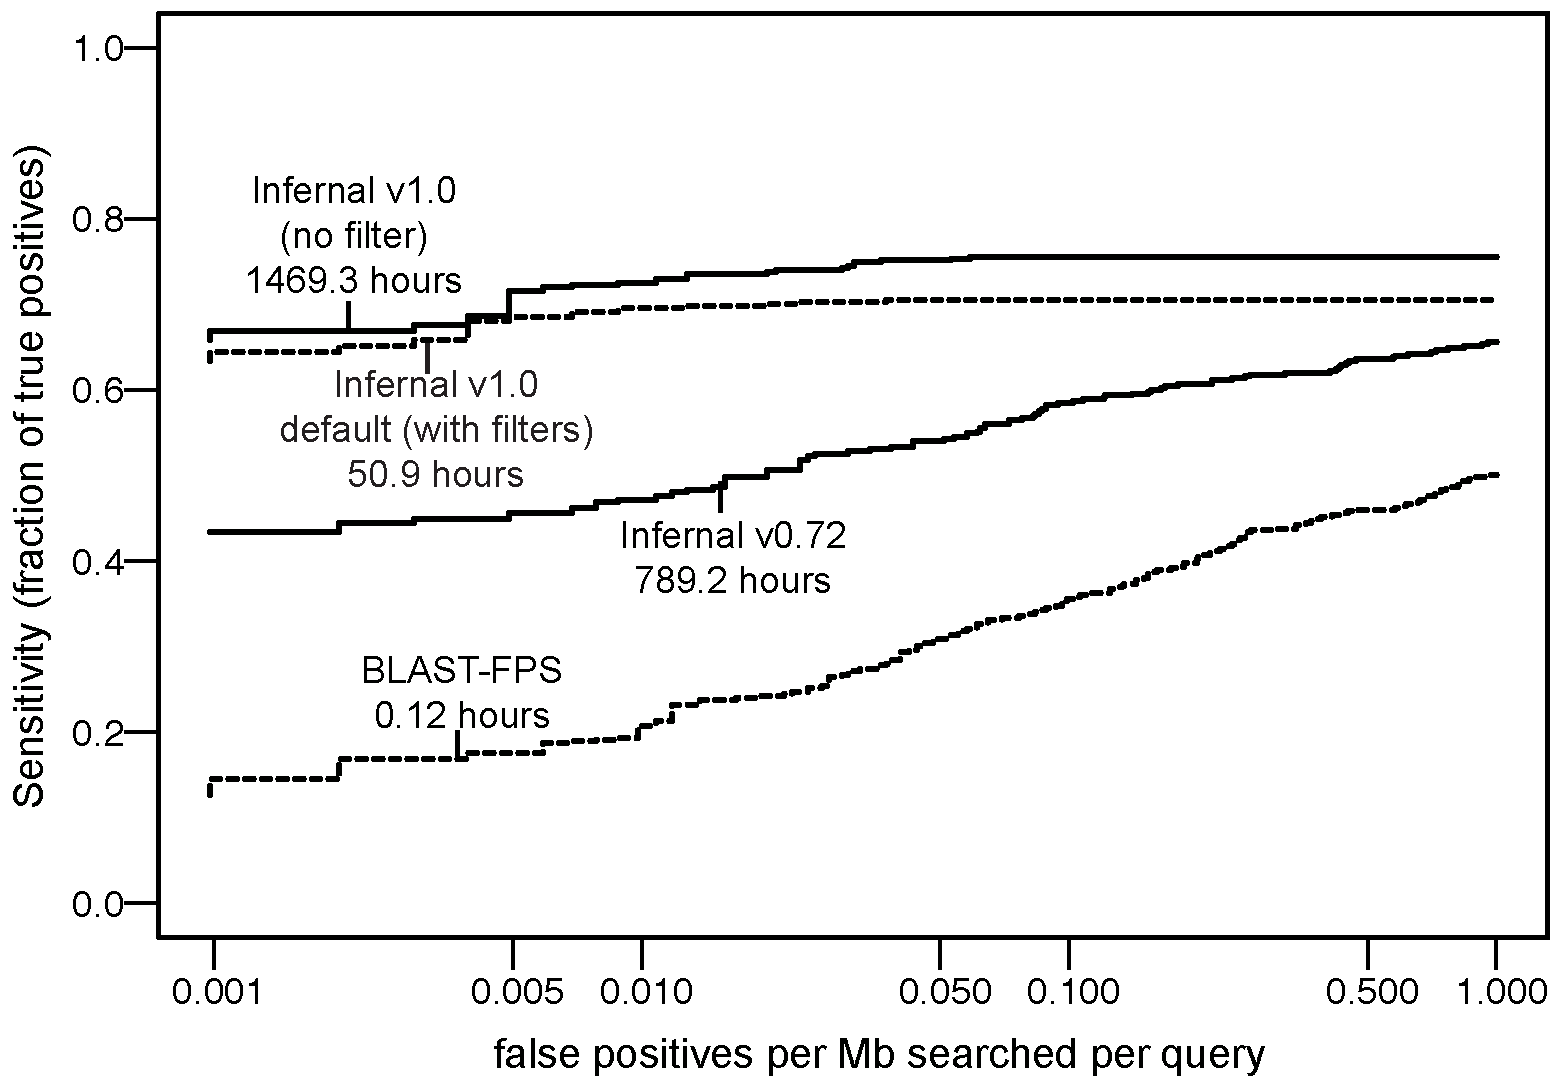
\includegraphics[width=6.4in]{figs/roc}
\caption{\textbf{ROC curves for the benchmark.}  Plots are shown for
the new \textsc{infernal} 1.0 with and without filters, for the old 
\textsc{infernal} 0.72, and for
family-pairwise-searches (FPS) with \textsc{blastn}.}
\label{fig:roc}
\end{center}
\end{figure}

\newpage

%%%%%%%%%%%%%%%%%%%%%%%%%%%%%%%%%%%%%%%%%%%%%%%%%%%%%%%%%%%%%%%%%%%%%%%
% The 6RNAs table, running times for various applications for 
% 6 RNAs
%\normalfont\ttfamily
\begin{table}
\begin{center}
\begin{tabular}{lrr|r|rr|r|} 
       & consensus & average \% id   & calibration  & \multicolumn{2}{c|}{search (min/Mb)} & alignment \\
family & length    & in training aln & (hours/model)& no filter & w/filters & (sec/seq) \\ \hline
tRNA    & 71       & 44\%            &       2.8h   &     47.3m &       8.7m&  0.013s \\
5S rRNA & 119      & 56\%            &       2.6h   &     58.6m &      10.1m&  0.026s \\
SRP RNA & 304      & 46\%            &      16.3h   &    333.7m &       5.6m&  0.168s \\
RNaseP  & 365      & 65\%            &      29.9h   &    408.9m &       1.7m&  0.176s \\
SSU rRNA& 1545     & 77\%            &      62.2h   &      n.d. &       n.d.&  1.087s \\
LSU rRNA& 2898     & 82\%            &     134.0h   &      n.d. &       n.d.&  3.072s \\
\end{tabular}
%
% alignment times (a subset of these will be in final table)
% 
% Timings from ~/notebook/8_0909_manuscript_inf-1_appnote/00LOG
% 
% family          & non-banded CYK & HMM banded CYK & HMM banded optacc (default)
%
% tRNA            &       0.049    &         0.0045 &            0.0129
% 5S rRNA         &       0.2023   &         0.0095 &            0.0256
% SRP RNA         &       5.4509   &         0.0615 &            0.1680
% RNase P         &      11.958    &         0.0721 &            0.1759
% SSU rRNA        &     724.201    &         0.7691 &            1.0870
% LSU rRNA        &   11819.9      &         2.5347 &            3.1206
%
%
% search times (a subset of these will be in final table)
% 
% Timings from ~/notebook/8_0909_manuscript_inf-1_appnote/00LOG
% times are per Mb (for forward AND reverse strand) on two input
% seq files: 10Mb.eq.fa   (25% A,C,G,U) = eq
% seq files: 10Mb.real.fa               = reall
% 
%                 ---------------------------------------------------------------------
% family          &    viterbi   &    forward    &     inside       &     filter      &
%                 ---------------------------------------------------------------------
%                 &   eq  & real & eq    & real  &  eq     &  real  &  eq    & real   & 
%                 ---------------------------------------------------------------------
% tRNA            &  6.8s & 6.8s & 20.5s & 20.5s &  2817.2s&  2840.7& 517.8s & 522.1s & 
% 5S rRNA         & 10.1s &10.0s & 32.1s & 32.0s &  3516.3 &  3517.5& 612.9s & 607.5s & 
% SRP RNA         & 22.6s &22.6s & 77.1s & 77.2s & 20099.3 & 20024.0& 878.9  & 335.3s &
% RNase P         & 26.9s &26.9s & 94.1s & 94.2s & 24533.3 & 24559.9& 124.1  & 103.3s &
% SSU rRNA        & 
% LSU rRNA        & 
%
\end{center}
\caption{\textbf{Calibration, search, and alignment running times for
    six known structural RNAs of various sizes.} SSU rRNA and LSU rRNA
    search times were not determined (n.d.); much faster non-CM
    methods are well suited for finding these RNAs, due to their high
    level of primary sequence conservation. CPU times are measured for
    single execution threads on otherwise unloaded 3.0 GHz Intel Xeon
    processors with 8 GB RAM, running Red Hat AS4 Linux operating
    systems.}
\label{tbl:times}
\end{table}

\end{document}



%%%%%%%%%%%%%%%%%%%%%%%%%%%%%%%%%%%%%%%%%%%%%%%%%%%%%%%%%%%
%%%%%%%%%%%%%%%%%%%%%%%%%%%%%%%%%%%%%%%%%%%%%%%%%%%%%%%%%%%
%%%%%%%%%%%%%%%%%%%%%%%%%%%%%%%%%%%%%%%%%%%%%%%%%%%%%%%%%%%

%%%%%%%%%%%%%%%%%%%%%%%%%%%%%%%%%%%%%%%%%%%%%%%%%%%%%%%%%%%
% OTHER POSSIBLE TABLES/FIGURES
%
% kept here for convenience in case they're needed later
%%%%%%%%%%%%%%%%%%%%%%%%%%%%%%%%%%%%%%%%%%%%%%%%%%%%%%%%%%%

%%%%%%%%%%%%%%%%%%%%%%%%%%%%%%%%%%%%%%%%%%%%%%%%%%%%%%%%%%%%%%%%%%%%%%%
% GC content figure 
%
\begin{comment}
\begin{figure}
\begin{center}
\includegraphics[width=6.4in]{figs/gc}
\caption{\textbf{GC content of 100 nucleotide windows in the
    benchmark pseudogenome and in a sampling of real genomic segments.}}  
\label{fig:gc-realmark}
\end{center}
\end{figure}
\end{comment}
%%%%%%%%%%%%%%%%%%%%%%%%%%%%%%%%%%%%%%%%%%%%%%%%%%%%%%%%%%%%%%%%%%%%%%%
% 6 RNAs table, different formatted
\begin{comment}
\begin{table}[htb]
\begin{center}
\begin{tabular}{ccccccr} 

       & consensus & \multicolumn{3}{c}{homology search} &  & alignment \\ \hline
family & length    & hmm & cm    & filtered & calibration   & sec/seq   \\ \hline
%                    fwd   inside non-banded
tRNA    & 71       & 20.5s & 3030s  & 522.1s   & 2.8h        & 0.013 \\
5S rRNA & 119      & 32.1s & 2941s  & 607.5s   & 2.6h        & 0.026 \\
SRP RNA & 304      & 77.2s & 25000s & 335.3s   & 16.3h       & 0.168 \\
RNaseP  & 365      & 94.1s & 50000s & 103.3s   & 29.9h       & 0.176 \\
SSU rRNA& 1545     &  ?    & ?      & ?        & 62.2h       & 1.087 \\
LSU rRNA& 2898     &  ?    & ?      & ?        & 134.0h      & 3.072 \\
\end{tabular}
\end{comment}
%%%%%%%%%%%%%%%%%%%%%%%%%%%%%%%%%%%%%%%%%%%%%%%%%%%%%%%%%%%%%%%%%%%%%%
% The rmark MER table - summary MERs
%\normalfont\ttfamily
\begin{comment}
\begin{table}[htb]
\begin{center}

\begin{tabular}{lccr} 

program & MER & hours \\ \hline
\textsc{blastn}                    & 286 &   0.02 \\
\textsc{infernal} 0.55             & 234 & 564.9  \\
\textsc{infernal} 0.72             & 185 &  84.0  \\
\textsc{infernal} 1.0 non-filtered & 109 & 159.0  \\
\textsc{infernal} 1.0 default      & 124 &  12.6  \\

\begin{tabular}{lccr} 

        & \multicolumn{2}{c}{MER} & \\
program & non-biased & biased & hours \\ \hline

\textsc{blastn}                    & 216 & 286 &   0.02 \\
\textsc{infernal} 0.55             & 232 & 234 & 564.9  \\
\textsc{infernal} 0.72             & 114 & 185 &  84.0  \\
\textsc{infernal} 1.0 non-filtered & 109 & 109 & 159.0  \\
\textsc{infernal} 1.0 default      & 120 & 124 &  12.6  \\

\end{tabular}
\end{center}
\caption{\textbf{Rfam benchmark MER summary statistics.}} 
\label{tbl:rmarkmerlist}
\end{table}
\end{comment}
%%%%%%%%%%%%%%%%%%%%%%%%%%%%%%%%%%%%%%%%%%%%%%%%%%%%%%%%%%%%%%%%%%%%%%%




